% !TEX root = main.tex

\section{理論}
\subsection{ROS 2とは}
ロボット技術は産業用から日常生活まで多岐にわたる応用が進んでおり,
それに伴い,開発の効率化やシステムの拡張性が求められている.
これらの課題に対応するため,オープンソースのロボットフレームワークである
ROS(Robot Operating System)が開発され,幅広い支持を得ている.
ROSは,通信,制御,センサーデータの統合など,ロボット開発における基盤となる機能を提供しており,
研究開発において重要な役割を果たしている.

ROS 2はDDS(Data Distribution Service)を通信基盤として採用している.
これにより,ノード間通信のリアルタイム性が向上し,
複数のロボットやセンサーから成る分散システムの構築が容易となった\cite{ros2design}.
特に,産業用ロボットや自動運転車のように,即時性が求められるシステムにおいて,その利点が顕著である.

さらに,クロスプラットフォーム対応もROS 2の特徴の一つである.
ROS 1は主にLinux環境での動作を前提としていたが,
ROS 2ではWindowsやmacOSなど複数のプラットフォームで動作するよう設計されており,
開発環境の柔軟性が大幅に向上した\cite{ros2docs}.
これにより,多様なハードウェア環境への適応が可能となり,利用者の裾野が広がった.

これらの特徴により,ROS 2は,
研究開発だけでなく商業用途にも適したフレームワークとして注目を集めている.
本研究においても,ROS 2を採用することで,効率的かつ信頼性の高いロボットシステムの開発を目指す.

\subsection{2輪ロボットの運動学}
2輪ロボットは,シンプルな構造でありながら,高い機動性を持つため,広く研究や産業に利用されている.
その運動学は,ロボットの速度制御や経路計画を行う上で不可欠な要素である.
本節では,2輪ロボットの運動学および逆運動学を導出する.

\begin{itemize}
    \item $v$:ロボットの並進速度 [m/s]
    \item $\omega$:ロボットの角速度 [rad/s]
    \item $r$:車輪の半径 [m]
    \item $L$:左右車輪間の距離 [m]
    \item $\dot{\theta}_R$,$\dot{\theta}_L$:右車輪および左車輪の角速度 [rad/s]
\end{itemize}
とする.

\begin{figure}[h]
    \centering
    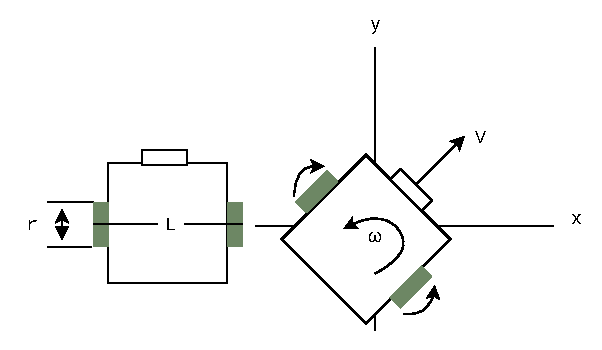
\includegraphics[width=0.5\textwidth]{figure/robot_model.pdf}
    \caption{2輪ロボットのモデル図}
    \label{fig:robot_model}
\end{figure}

\subsubsection{順運動学}
順運動学では,各車輪の角速度$\dot{\theta}_R$および$\dot{\theta}_L$から,ロボットの並進速度$v$,角速度$\omega$,および自己位置を算出する.自己位置の計算は,ロボットの進行方向と回転を考慮して行う.

ロボットの並進速度$v$と角速度$\omega$は,次式で表される.
\begin{equation}
    v = \frac{r}{2} (\dot{\theta}_R + \dot{\theta}_L)
    \label{eq:forward_v}
\end{equation}
\begin{equation}
    \omega = \frac{r}{L} (\dot{\theta}_R - \dot{\theta}_L)
    \label{eq:forward_omega}
\end{equation}

これに基づき,ロボットの自己位置$(x, y)$と向き$\theta$の時間変化を次のように表す.
\begin{equation}
    \dot{x} = v \cos \theta
    \label{eq:forward_x}
\end{equation}
\begin{equation}
    \dot{y} = v \sin \theta
    \label{eq:forward_y}
\end{equation}
\begin{equation}
    \dot{\theta} = \omega
    \label{eq:forward_theta}
\end{equation}

これらの微分方程式を離散化することで,時刻$t_k$における位置と向きを計算することができる.離散化した式は次のようになる.
\begin{equation}
    x_{k+1} = x_k + v_k \cos \theta_k \Delta t
    \label{eq:discrete_x}
\end{equation}
\begin{equation}
    y_{k+1} = y_k + v_k \sin \theta_k \Delta t
    \label{eq:discrete_y}
\end{equation}
\begin{equation}
    \theta_{k+1} = \theta_k + \omega_k \Delta t
    \label{eq:discrete_theta}
\end{equation}
ここで,$\Delta t$は計算ステップの時間間隔を示す.

\subsubsection{逆運動学}
逆運動学では,ロボットの並進速度$v$と角速度$\omega$から,
車輪の角速度$\dot{\theta}_R$および$\dot{\theta}_L$を求める.
ロボットの基本的なモデルを図\ref{fig:robot_model}に示す.

ロボットの並進速度$v$および角速度$\omega$は,
車輪の角速度$\dot{\theta}_R$および$\dot{\theta}_L$により次式で表される.
\begin{equation}
    v = \frac{r}{2} (\dot{\theta}_R + \dot{\theta}_L)
    \label{eq:v}
\end{equation}
\begin{equation}
    \omega = \frac{r}{L} (\dot{\theta}_R - \dot{\theta}_L)
    \label{eq:omega}
\end{equation}

式\eqref{eq:v}および式\eqref{eq:omega}を連立すると,次のように導出できる.
\begin{equation}
    \dot{\theta}_R = \frac{1}{r} (v + \frac{L}{2} \omega)
    \label{eq:theta_R}
\end{equation}
\begin{equation}
    \dot{\theta}_L = \frac{1}{r} (v - \frac{L}{2} \omega)
    \label{eq:theta_L}
\end{equation}

これらの式により,目標速度$v$と$\omega$が与えられた場合に,
車輪の角速度$\dot{\theta}_R$と$\dot{\theta}_L$を算出し,ロボットの各車輪を制御できる.

\subsection{PID制御とローパスフィルタ}
PID制御(Proportional-Integral-Derivative Control)は,
制御工学における最も基本的かつ広く使用されているフィードバック制御の手法である.
本節では,PID制御の基本構造とローパスフィルタについて説明する.

\subsubsection{PID制御の構造}
PID制御は,目標値と現在値の偏差を基に制御量を算出し,システムを目標値へ収束させる手法である.
制御量$u(t)$は次式で定義される:
\begin{equation}
    u(t) = K_P e(t) + K_I \int_{0}^{t} e(\tau) d\tau + K_D \frac{de(t)}{dt}
    \label{eq:pid}
\end{equation}
ここで,
\begin{itemize}
    \item $e(t)$:目標値と現在値の偏差
    \item $K_P$:比例ゲイン(P制御)
    \item $K_I$:積分ゲイン(I制御)
    \item $K_D$:微分ゲイン(D制御)
\end{itemize}
各項の役割は以下の通りである.
\begin{itemize}
    \item 比例制御(P制御):偏差に比例した制御量を生成し,応答の速さを向上させる.
    \item 積分制御(I制御):偏差を累積することで,定常偏差を排除する.
    \item 微分制御(D制御):偏差の変化率を基に,過渡応答の振動を抑制する.
\end{itemize}

\begin{figure}[h]
    \centering
    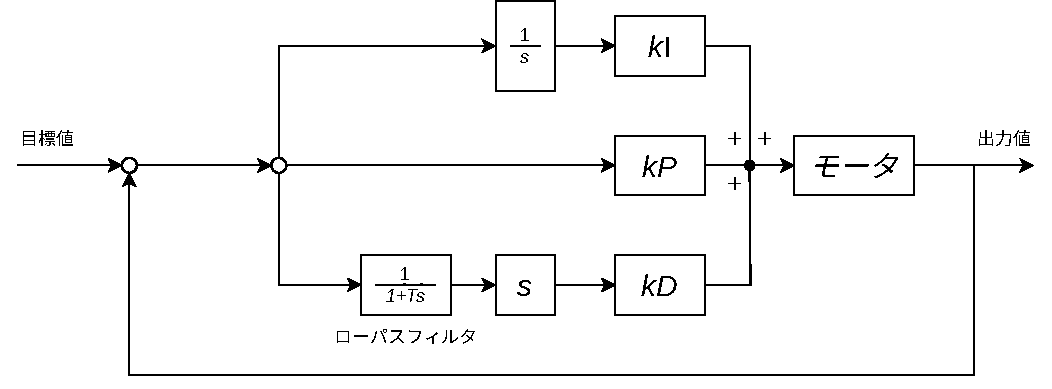
\includegraphics[width=0.7\textwidth]{figure/pid.pdf}
    \caption{PID制御器の構成図}
    \label{fig:pid_controller}
\end{figure}

図\ref{fig:pid_controller}にPID制御器の構成図を示す.
本研究では,このPID制御器を用いてロボットの各車輪の速度を制御している.

\subsubsection{ローパスフィルタの導入}
微分制御(D制御)は高周波ノイズに敏感であり,そのまま使用するとシステムの安定性を損なう可能性がある.
この問題を軽減するために,微分項にローパスフィルタを適用することが一般的である.

ローパスフィルタを適用した微分制御項は次式で表される:
\begin{equation}
    D(s) = \frac{K_D s}{1 + T s}
    \label{eq:lowpass_filter}
\end{equation}
ここで,
\begin{itemize}
    \item $T$:カットオフ周波数
\end{itemize}

ノイズが,微分により増幅されるが,1次遅れ系であるローパスフィルターにより,ノイズの影響が軽減される.

\subsection{YOLOv5による物体認識}
本研究では,人の認識にYOLOv5(You Only Look Once Version 5)を使用する.
YOLOはリアルタイムで物体を検出するアルゴリズムであり,
1枚の画像に対して物体のクラスとその位置を同時に出力する特徴を持つ.
単一のニューラルネットワークを用いて,画像内の物体のバウンディングボックスとクラスラベルを直接予測する\cite{yolo}.
そのため他の物体検出モデル(例えばSSDやFaster R-CNN)と比較して,
高速な推論速度と高い精度を両立している.このため,リアルタイム性が要求されるロボットシステムにおいて有用である.

本研究では,YOLOv5を用いてデプスカメラD435iから得られたRGB画像内の人を認識する.
YOLOv5は以下のステップで物体を検出する.
\begin{enumerate}
    \item RGB画像を入力し,YOLOv5のバックボーンにより特徴を抽出する.
    \item ネックでスケールを調整し,特徴を統合する.
    \item ヘッドでバウンディングボックス,クラスラベル(人),および信頼度スコアを出力する.
\end{enumerate}

出力されたバウンディングボックスは,ピクセル座標で記述されており,
これをデプスカメラのデプスマップと組み合わせることで,物理座標を算出する.


\subsection{デプスデータからの人座標検出}
デプスカメラは,対象物までの距離を計測するためのデバイスであり,ロボットの環境認識や障害物回避,
物体追跡などの応用において重要な役割を果たす.
本研究では,インテル® RealSense™ デプスカメラ D435iを使用し,
カメラから取得したデプスデータを基に人追従アルゴリズムを実現する.
\begin{figure}[h]
    \centering
    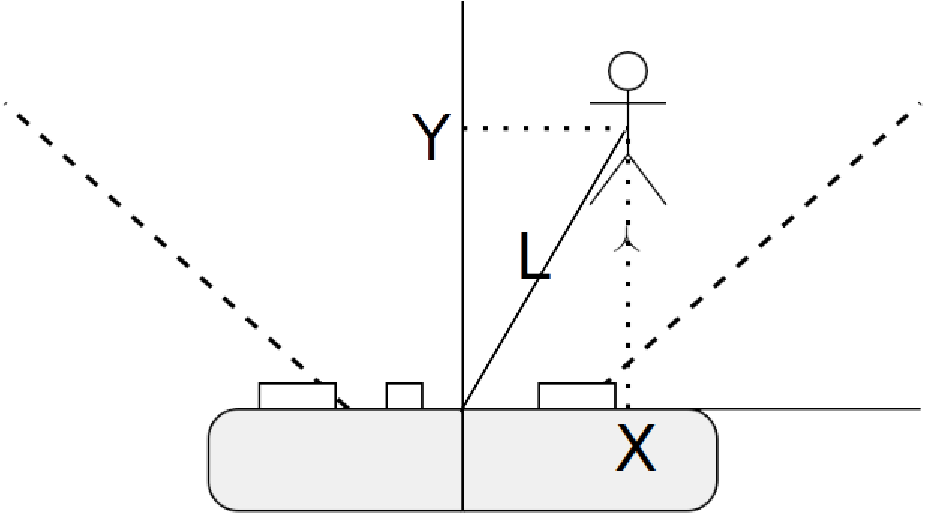
\includegraphics[width=0.4\textwidth]{figure/rialsens_man.pdf}
    \caption{デプスカメラを用いた座標変換モデル}
    \label{fig:coordinate_conversion}
\end{figure}

デプスカメラで取得したデータを用いて,画像上のピクセル座標を実空間の物理座標に変換することで,人の位置を検出する.図\ref{fig:coordinate_conversion}に示すように,ピクセル座標系における対象物の位置を,カメラ座標系に変換する手順を以下に述べる.

デプスカメラのデプスマップは,各ピクセルに深度情報$L$(対象物までの斜距離)を格納している.この情報を用いて,画像座標系におけるピクセル座標$(u, v)$をカメラ座標系$(X_c, Y_c)$に変換する.なお,本実験では上下方向($Z$軸)は考慮しない.

変換には以下の式を使用する.
\begin{equation}
    X_c = \frac{(u - c_x) \cdot L}{f_x}
    \label{eq:xc}
\end{equation}
\begin{equation}
    Y_c \approx L
    \label{eq:yc}
\end{equation}
ここで,$u$および$v$は画像座標系のピクセル位置,$c_x$はカメラの光学中心(水平方向の画面中心)のピクセル位置,$f_x$はカメラの焦点距離(ピクセル単位),$L$はデプスマップから取得される深度値(対象物までの斜距離)である.

次に,カメラ座標系における2次元位置$(X_c, Y_c)$をロボット座標系$(X_r, Y_r)$に変換する.この変換は,カメラとロボット間の座標系の相対的な位置関係を記述する回転行列$R$と平行移動ベクトル$T$を用いることで行われる.

ロボット座標系への変換は,次の行列式で表される.
\begin{equation}
    \begin{bmatrix}
        X_r \\ Y_r \\ 1
    \end{bmatrix}
    =
    \begin{bmatrix}
        R & T \\ 
        0 & 1
    \end{bmatrix}
    \begin{bmatrix}
        X_c \\ Y_c \\ 1
    \end{bmatrix}
    \label{eq:transform}
\end{equation}

ここで,
\begin{itemize}
    \item $R$:カメラ座標系からロボット座標系への回転行列
    \item $T$:カメラ座標系からロボット座標系への平行移動ベクトル
\end{itemize}

本実験では,カメラがロボットに平行に取り付けられているため,回転行列$R$は単位行列として扱う.
また,カメラがロボットの旋回中心から$200\ \mathrm{mm}$($0.2\ \mathrm{m}$)前方に取り付けられているため,
平行移動ベクトル$T$は以下のように与えられる.
\begin{equation}
    T = \begin{bmatrix} 0.0 \\ 0.2 \end{bmatrix}
\end{equation}

実際に計算例を示す.以下のパラメータを仮定する.
\begin{itemize}
    \item デプスカメラの焦点距離:$f_x = 378.09$ [px]
    \item デプスカメラの光学中心:$c_x = 319.39$ [px]
    \item デプスマップからの深度値:$L = 2.5$ [m]
    \item 対象物の水平ピクセル座標:$u = 400$ [px]
    \item カメラ位置のオフセット:$T_x = 0.2$ [m]
\end{itemize}

まず,画像座標系でのズレ$\Delta u$を計算する.
\begin{equation}
    \Delta u = u - c_x = 400 - 319.39 = 80.61 \, \text{[px]}
\end{equation}

次に,カメラ座標系での水平座標$X_c$を求める.
\begin{equation}
    X_c = \frac{\Delta u \cdot L}{f_x} = \frac{80.61 \cdot 2.5}{378.09} \approx 0.534 \, \text{[m]}
\end{equation}

奥行き$Y_c$を近似的に求める.
\begin{equation}
    Y_c \approx L = 2.5 \, \text{[m]}
\end{equation}

最後に,ロボット座標系での位置$(X_r, Y_r)$を計算する.
\begin{equation}
    X_r = X_c + T_x = 0.534 +0 = 0.534 \, \text{[m]}
\end{equation}
\begin{equation}
    Y_r = Y_c + T_y = 2.5 + 0.2 = 4.5 \, \text{[m]}
\end{equation}

この計算により,目標物のロボット座標系における位置が得られる.

\subsection{人追従アルゴリズム}

\subsubsection{比例航法 (Proportional Navigation, PN)}
比例航法は,目標物(人物)の追従において,距離と偏差(横方向のズレ)を用いて
制御信号を生成する基本的なアルゴリズムである.本来であれば,目標までの視線角度をもとに計算するが,簡易化のため,横方向のズレを使用する.
以下に,本実験で使用する比例航法の式を示す.

\begin{align}
    V      & = k_v \cdot (P_d - 1.0)                     \\
    \omega & = k_\omega \cdot \frac{P_o}{\max(P_d, 1.0)}
\end{align}
\begin{itemize}
    \item \(k_v\):並進速度の比例ゲイン
    \item \(k_\omega\):角速度の比例ゲイン
    \item \(P_d\):ロボットと目標間の距離
    \item \(P_o\):横方向の偏差
\end{itemize}

しかしながら,比例航法では対象までの距離が近づくにつれ横方向の偏差の変化が大きくなりロボットが振動的になると考えられる.
そこで次の修正比例航法を提案する.

\subsubsection{修正比例航法 (Modified Proportional Navigation, MPN)}
比例方法では,大きな変化に対して大きな出力となり,ロボットの動きが激しくなってしまう.
そこで修正比例航法では,偏差の変化率(偏差角速度)を考慮することで,
ロボットの動作をより滑らかにする.
偏差角速度は以下の式で計算される.
\begin{equation}
    \dot{e}(k) = \frac{P_o(k) - P_o(k-1.0)}{\Delta t}
\end{equation}
角速度 \(\omega\) は以下の式で修正される.
\begin{equation}
    \omega(k) = k_\omega \cdot \frac{P_o(k)}{\max(P_d(k), 1.0)} + \lambda \cdot \dot{e}(k)
\end{equation}
ここで,
\begin{itemize}
    \item \(\lambda\):偏差角速度に対するゲイン
    \item \(\Delta t\):制御周期
\end{itemize}

これにより,急激な方向転換や不安定な動作が軽減され,滑らかな動作が可能となる.

\subsubsection{ゲインスケジューリング修正比例航法
    (Gain-Scheduled Modified Proportional Navigation, GS-MPN)}
ゲインスケジューリング修正比例航法では,偏差角速度に基づき動的なゲインスケジューリングを導入する.

動的微分ゲイン \(k_d\) は以下の式で定義される.
\begin{equation}
    k_d = \lambda_d \cdot \frac{1 - \exp(-a \cdot |\dot{\text{offset}}|)}{1 + \exp(-a \cdot |\dot{\text{offset}}|)}
\end{equation}
\begin{itemize}
    \item \(\lambda_d\):微分ゲインの最大値
    \item \(a\):微分ゲインの変化速度を調整するパラメータ
\end{itemize}

\begin{figure}[H]
    \centering
    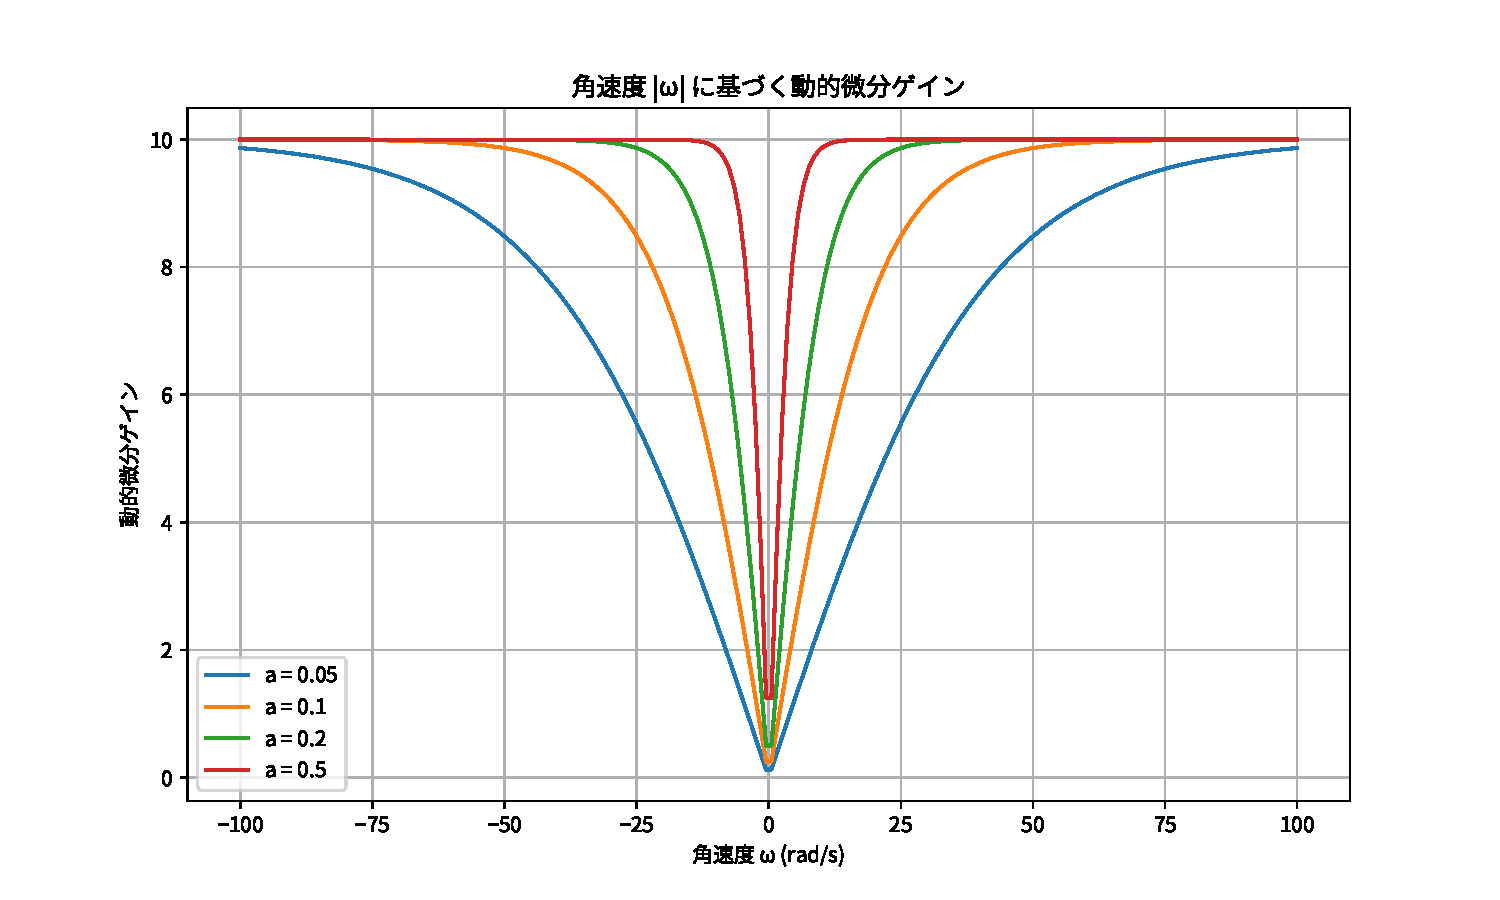
\includegraphics[width=0.7\textwidth]{figure/dynamicgain.pdf}
    \caption{動的微分ゲイン}
    \label{fig:dynamicgain}
\end{figure}
また,図\ref{fig:dynamicgain}に角速度に基づく動的微分ゲインのグラフを示す.

角速度 \(\omega\) は次式で計算される.
\begin{equation}
    \omega = k_\omega \cdot \frac{\text{person\_offset}}{\max(\text{person\_distance}, 1.0)} + k_d \cdot \dot{\text{offset}}
\end{equation}

